\section{INVERSE FUNCTION OF AN (H) FUNCTION}

If \(f\) is an (H) function, then \(f\) is monotone and continuous on an interval \([x_0, +\infty[\) , so the inverse function \(\varphi\) of the restriction of \(f\) to this interval is monotone and continuous on a neighbourhood of the point \(a = \lim_{x \to +\infty} f(x)\) ; but, if \(a\) is equal to \(+\infty\) (resp. \(-\infty\) , finite), one can show that \(\varphi(y)\) (resp. \(\varphi(-y)\) , \(\varphi(a + \frac{1}{y})\) or \(\varphi(a - \frac{1}{y})\) ) is not in general equal to an (H) function on a neighbourhood of \(+\infty\) . Nevertheless we shall see that in certain important cases one can obtain an (H) function equivalent to \(\varphi(y)\) (resp. \(\varphi(-y)\) , \(\varphi(a + \frac{1}{y})\) , \(\varphi(a - \frac{1}{y})\) ) and sometimes even an asymptotic expansion of this function relative to the scale \(\mathcal{E}\) defined in V, p.~254.

We shall use the following proposition:

PROPOSITION 4. Let \(p\) and \(q\) be two (H) functions which are strictly positive on an interval \([x_0, +\infty[\) .

\(1^{\circ}\) If \(q \ll p / p'\) one has \(p(x + q(x)) \sim p(x)\) .

\(2^{\circ}\) If both \(q \prec p/p'\) and \(q(x) \prec x\) then \(p(x - q(x)) \sim p(x)\) .

The two parts of this proposition are clear if \(p \sim k\) (constant \(\neq 0\) ); one may therefore suppose that \(p(x) \ll 1\) (otherwise one applies the argument to \(1/p\) ). One then deduces \(p'(x) \ll 1\) .

\(1^{\circ}\) One can write \(p(x + q(x)) = p(x) + q(x)p'(x + \theta q(x))\) with \(0 \leqslant \theta \leqslant 1\) (I, p.~14, corollary). Since \(\left|p'(x)\right|\) tends to 0 as \(x\) tends to \(+\infty\) , and is equal to an (H) function on a neighbourhood of \(+\infty\) , it is decreasing on an interval \([x_1, +\infty[\) , so, for \(x \geqslant x_1\) , one has \(\left|p'(x + \theta q(x))\right| \leqslant \left|p'(x)\right|\) ; since \(qp' \ll p\) one has \(p(x + q(x)) \sim p(x)\) .

\(2^{\circ}\) The condition \(q(x) \ll x\) ensures that \(x - q(x)\) tends to \(+\infty\) with \(x\) . Again one has \(p(x - q(x)) = p(x) - q(x)p'(x - \theta p(x))\) with \(0 \leqslant \theta \leqslant 1\) . The same argument as in the first part of the proof shows that, for \(x\) sufficiently large, \(\left|p'(x - \theta q(x))\right| \leqslant \left|p'(x - q(x))\right|\) . It reduces to showing that \(q(x)\frac{p'(x - q(x))}{p(x - q(x))}\) tends to 0 as \(x\) tends to \(+\infty\) . The proposition is true if \(p'/p \gg 1\) since then \(\left|p'/p\right|\) is an (H) function, increasing for \(x\) large enough; thus \(q(x)\frac{\left|p'(x - q(x))\right|}{\left|p(x - q(x))\right|} \leqslant q(x)\frac{\left|p'(x)\right|}{\left|p(x)\right|}\) , and \(qp' \ll p\) by hypothesis. It is also true if \(p'/p \sim k\) ( \(k\) constant \(\neq 0\) ), for then

\[
\frac {p ^ {\prime} (x - q (x))}{p (x - q (x))} \sim \frac {p ^ {\prime} (x)}{p (x)}
\]

since \(x - q(x)\) tends to \(+\infty\) . It only remains to examine the case where \(p' / p \ll 1\) . First suppose that \(p(x)\) is of finite order relative to x, and so (V, p.~232, prop. 7) \(p'(x) / p(x) \ll 1 / x\) . Then one has

\[
\frac {p ^ {\prime} (x - q (x))}{p (x - q (x))} = \frac {1}{x - q (x)} O _ {1} (1),
\]

so

\[
q (x) \frac {p ^ {\prime} (x - q (x))}{p (x - q (x))} = \frac {q (x)}{x} \left(1 - \frac {q (x)}{x}\right) ^ {- 1} O _ {1} (1) = \frac {q (x)}{x} O _ {2} (1),
\]

and one sees in this case that the proposition is true subject only to the hypothesis that \(q(x) \ll x\) . Finally we examine the case where \(1/x \ll p'(x)/p(x) \ll 1\) ; the function \(r = p'/p\) is then of finite order relative to x; since, by the preceding remark, prop.4 of V, p.255, is applicable to such a function, one has \(p'(x-q(x))/p(x-q(x)) \sim p'(x)/p(x)\) , and the hypothesis \(qp' \ll p\) allows us to complete the proof.

Remark. The conditions imposed on \(q(x)\) may not be improved, as the following examples show:

\begin{enumerate}
\def\labelenumi{\alph{enumi})}
\tightlist
\item
\end{enumerate}

\[
p (x) = e ^ {x}, \qquad q (x) = 1 = \frac {p (x)}{p ^ {\prime} (x)}, \qquad p (x + q (x)) = e p (x)
\]

\begin{enumerate}
\def\labelenumi{\alph{enumi})}
\setcounter{enumi}{1}
\tightlist
\item
\end{enumerate}

\[
\begin{array}{c} p (x) = \log x, \qquad q (x) = x - \log x \ll \frac {p (x)}{p ^ {\prime} (x)} = x \log x, \\ p (x - q (x)) = \log \log x \ll p (x). \end{array}
\]

We shall first study the inverses of (H) functions of a particular sort:

PROPOSITION 5. Let g be an (H) function not equivalent to a constant \(\neq 0\) , and such that \(g(x) \prec x\) , and let \(u(x)\) be the inverse function of \(x - g(x)\) , defined on a neighbourhood of \(+\infty\) . Let \((u_n)\) be the sequence of functions defined, by recursion on n, by the conditions \(u_0(x) = x\) , \(u_n(x) = x + g(u_{n-1}(x))\) for \(n \geqslant 1\) ; then \(u_n \gg 1\) and

\[
u (x) - u _ {n} (x) \sim g (x) \left(g ^ {\prime} (x)\right) ^ {n}.\tag{11}
\]

Let us put \(y = u(x)\) , \(y_{n} = u_{n}(x)\) ; then \(x = y - g(y)\) , \(y_{0} = x\) and \(y_{n} = x + g(y_{n+1})\) . One first deduces that \(x/y = 1 - \frac{g(y)}{y}\) ; since y tends to \(+\infty\) with x, the hypothesis \(g(x) \ll x\) shows that \(y = u(x) \sim x = y_{0}\) ; further,

\[
y - x = g (y) = g (x) + (y - x) g ^ {\prime} (z)
\]

where z belongs to the interval with endpoints x, y; when x tends to \(+\infty\) so does z, and since \(g(x) \ll x\) , \(g' \ll 1\) , thus \(g'(z)\) tends to 0, and consequently

\[
y - x = g (x) + o (y - x)
\]

whence

\[
u (x) - x \sim g (x).\tag{12}
\]

In the second place we show, by recursion on \(n\) , that when \(x\) tends to \(+\infty\) one has \(u_{n} \gg 1\) , and

\[
u (x) - u _ {n} (x) \prec u (x) - u _ {n - 1} (x).\tag{13}
\]

Indeed, \(y - y_{n} = g(y) - g(y_{n-1}) = (y - y_{n-1})g'(z_{n-1})\) , where \(z_{n-1}\) belongs to the interval with endpoints y and \(y_{n-1}\) ; by the induction hypothesis \(z_{n-1}\) tends to \(+\infty\) with x, and so \(g'(z_{n-1})\) tends to 0, which proves (13). One deduces from this relation and from (12) that \(u(x) - u_{n}(x) \ll u(x) - x \sim g(x) \ll x \sim u(x)\) , whence \(u_{n}(x) \sim u(x)\) and consequently \(u_{n} \gg 1\) . Finally, the relation \(u(x) - u_{n}(x) \ll u(x) - x\) can also be written \((u(x) - x) - (u_{n}(x) - x) \ll u(x) - x\) , whence

\[
u _ {n} (x) - x \sim u (x) - x \sim g (x).\tag{14}
\]

To prove (11), first remark that if \(t(x)\) is a function such that \(t(x) - x \sim g(x)\) , then one has \(g'(t(x)) \sim g'(x)\) . Indeed, for any \(\varepsilon > 0\) , for x sufficiently large \(g'\) is monotone, so \(g'(t(x))\) lies between \(g'(x + (1 + \varepsilon)g(x))\) and \(g'(x + (1 - \varepsilon)g(x))\) . Prop. 4 of V, p.~255, shows that \(g'(t(x)) \sim g'(x)\) , provided one has established the relation \(g \ll g'/g''\) . Now, if g is of infinite order relative to x one has (V, p.~251, prop. 2) \(g''/g' \sim g'/g\) , and, since \(g' \ll 1\) , \(g \ll g/g' \sim g'/g''\) ; if g is of finite order \(\mu\) relative to x one necessarily has \(\mu \leqslant 1\) ; if \(\mu < 1\) , since g is not equivalent to a constant \(\neq 0\) , formulae (3) and (4) (V, p.~251) show that \(g''/g' \sim k/x\) (k constant \(\neq 0\) ), whence again \(g \ll g'/g''\) ; finally, if \(\mu = 1\) then \(g'\) is of order 0 relative to x, so \(g''/g' \ll 1/x\) , and so again \(g \ll g'/g''\) .

This being so, since \(z_{n-1}\) lies between \(y\) and \(y_n\) , it follows from (14) that \(z_{n-1} - x \sim g(x)\) , whence \(g'(z_{n-1}) \sim g'(x)\) by the above; thus

\[
y - y _ {n} \sim (y - y _ {n - 1}) g ^ {\prime} (x),
\]

whence we obtain (11) by induction on \(n\) .

Remarks. 1) If \(g\) is of order \(< 1\) relative to \(x\) , the function \(u(x) - u_n(x)\) tends to 0 with \(x\) once \(n\) is sufficiently large. Indeed, in the opposite case one would have \(gg'^n \gg 1\) for every \(n\) , so \(g\) would be of infinite order relative to \(1 / g'\) ; in other words, one would have \(\log |g| \gg \log |g'|\) , whence, on differentiating, \(g'/g \gg g''/g'\) . But if \(g\) is of order \(\mu < 1\) relative to \(x\) one has \(g'/g \sim g''/g'\) when \(\mu = -\infty\) , \(\frac{g'}{g} \sim \frac{\mu}{\mu - 1} \frac{g''}{g'}\) when \(\mu \neq 0\) , and finally \(g'/g \ll g''/g'\) when \(\mu = 0\) (V, p.~251, n° 3).

In contrast, if \(g\) is of order 1 relative to \(x\) one can have \(gg'^n \gg 1\) for every integer \(n > 0\) , as the example \(g(x) = x / \log x\) shows.

\begin{enumerate}
\def\labelenumi{\arabic{enumi})}
\setcounter{enumi}{1}
\tightlist
\item
  When \(g(x)\) is an (H) function equivalent to a constant \(k \neq 0\) one has \(g(x) = k + g_1(x)\) , with \(g_1 \ll 1\) ; the function \(u_1(x) = u(x) - k\) is the inverse of the function \(x - g_1(x + k)\) , and one is brought back to the case treated in prop. 5 of V, p.~256.
\end{enumerate}

To have an asymptotic expansion for the function u it thus suffices to have such an expansion for the function \(u_{n}\) : if g admits an asymptotic expansion relative to the scale under consideration one is thus led (by the definition of (H) functions) to the problems examined in V, p.~223 to 227.

The most general case, as follows, reduces to the case treated in prop. 5 of V, p.~256: the function \(y = u(x)\) is assumed to satisfy the relation

\[
\varphi (x) = \psi (y) - g (y)\tag{15}
\]

where \(\varphi\) is an (H) function, \(\psi\) is an (H) function such that \(\psi \gg 1\) and such that the inverse function \(\theta\) of \(\psi\) is also an (H) function, and g is an (H) function such that \(g \ll \psi\) . Let now \(v(x)\) be the inverse function of \(x - g(\theta(x))\) ; one has \(u = \theta \circ v \circ \varphi\) , and \(g(\theta(x)) \ll x\) ; if one knows an asymptotic expansion for v thanks to prop. 5 of V, p.~256, one can then deduce an asymptotic expansion for u as in V, p.~223 to 227.

Examples. 1) Let us seek an asymptotic expansion for the inverse function \(v(x)\) of \(x^{5} + x\) (for x tending to \(+\infty\) ); putting \(x^{5} = t\) one is led to seek an expansion of the inverse function \(u(t)\) of \(t + t^{1/5}\) (for t tending to \(+\infty\) ), that is, to apply prop. 5 of V, p.~256, to the case where \(g(t) = -t^{1/5}\) . Let us, for example, calculate, \(u_{2}(t)\) ; one has

\[
u _ {2} (t) = t - \left(t - t ^ {1 / 5}\right) ^ {1 / 5} = t - t ^ {1 / 5} + \frac {1}{5} t ^ {- 3 / 5} + \frac {2}{2 5} t ^ {- 7 / 5} + o _ {1} \left(t ^ {- 7 / 5}\right).
\]

Moreover, by (11) (V, p.~256)

\[
u (t) - u _ {2} (t) \sim - \frac {1}{2 5} t ^ {- 7 / 5}
\]

whence

\[
u (t) = t - t ^ {1 / 5} + \frac {1}{5} t ^ {- 3 / 5} + \frac {1}{2 5} t ^ {- 7 / 5} + o _ {2} \left(t ^ {- 7 / 5}\right)
\]

and one deduces the expansion

\[
v (x) = u (x) ^ {1 / 5} = x ^ {1 / 5} - \frac {1}{5} x ^ {- 3 / 5} - \frac {1}{2 5} x ^ {- 7 / 5} + o _ {3} \left(x ^ {- 7 / 5}\right)
\]

sought.

\begin{enumerate}
\def\labelenumi{\arabic{enumi})}
\setcounter{enumi}{1}
\tightlist
\item
  Let us seek an asymptotic expansion for the inverse function of the function \(x/\log x\) ; from the identity \(x = y/\log y\) , where \(y = v(x)\) , one deduces \(\log x = \log y - \log \log y\) ; on putting \(z = \log y\) , \(t = \log x\) , one has \(t = z - \log z\) , and one is led to expand the inverse function \(u(t)\) of \(t - \log t\) ; for example, one has
\end{enumerate}

\[
u _ {2} (t) = t + \log (t + \log t) = t + \log t + \frac {\log t}{t} - \frac {(\log t) ^ {2}}{2 t ^ {2}} + o _ {1} \left(\frac {\log t}{t ^ {2}}\right)
\]

and moreover, by (11) (V, p.~256)

\[
u (t) - u _ {2} (t) \sim \frac {\log t}{t ^ {2}}
\]

whence

\[
u (t) = t + \log t + \frac {\log t}{t} - \frac {(\log t) ^ {2}}{2 t ^ {2}} + \frac {\log t}{t ^ {2}} + o _ {2} \left(\frac {\log t}{t ^ {2}}\right)
\]

and on returning to the original problem one obtains the asymptotic expansion

\[
v (x) = x \log x + x \log \log x + x \frac {\log \log x}{\log x} + o \left(x \frac {\log \log x}{\log x}\right).
\]

\pandocbounded{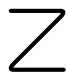
\includegraphics[keepaspectratio]{images/part002_15bf1a92.jpg}}

Remark. Note that two equivalent (H) functions can have non-equivalent inverses, as the example of the two functions \(\log x\) and \(1 + \log x\) shows.

\setcounter{exercisegroup}{0}
\refstepcounter{exercisegroup}
